\subsection{Algoritmy vyhledávání v textu}
Toto sú len veľmi stručné výťahy z wikipedie. Aktuálne sú tu len preto, aby si človek rýchlo vybavil, o čom tie algoritmy sú :-)

\subsubsection*{Rabin-Karp}
Umožňuje vyhľadávanie viacerých reťazcov v texte naraz - užitočné napr. na hľadanie plagiátov. Základnou myšlienkou je vyhľadávanie v texte pomocou hashov (rolling hashes - idea je \texttt{s[i+1..i+m] = s[i..i+m-1] - s[i] + s[i+m]})...

Algoritmus pre vyhľadávanie jedného reťazca:
\begin{verbatim}
 1 function RabinKarp(string s[1..n], string sub[1..m])
 2     hsub := hash(sub[1..m])
 3     hs := hash(s[1..m])
 4     for i from 1 to n-m+1
 5         if hs = hsub
 6             if s[i..i+m-1] = sub
 7                 return i
 8         hs := hash(s[i+1..i+m])
 9     return not found
\end{verbatim}

Najhoršia zložitosť je $\Omega(mn)$. Pri vyhľadávaní viacerých reťazcov len spočítame hashe všekých hľadaných stringov a pri nájdení niektorého z hashov príslušný reťazec porovnáme s textom... Ostatné algoritmy spotrebujú čas $O(n)$ na nájdenie 1 reťazca a teda $O(nk)$ na vyhľadanie $k$ reťazcov. Naproti tomu tento algoritmus má očakávanú zložitosť $O(n+k)$ - pretože vyhľadávanie v hashovacej tabuľke, či je hash podreťazca textu rovný hashu niektorého z hľadaného reťazcov, trvá $O(1)$.

\subsubsection*{Aho-Corasick}

Dokáže vyhľadávať viacero reťazcov naraz - používa na to trie-like štruktúru (konečný automat), ktorý obsahuje nasledujúce \uv{prvky}:
\begin{penumerate}
	\item konečná množina $Q$ - stavy
	\item konečná abeceda $A$
	\item transition funkcia $g$: $Q \times A \rightarrow Q + \{fail\}$
	\item failure funkcia $h$: $Q \rightarrow Q + \{fail\}$. $h(q)=q'$ práve vtedy keď spomedzi všetkých stavov Q dáva $q'$ najdlhší suffix z $path(q)$.
	\item konečná množina $F$ - koncové stavy
\end{penumerate}

Príklad \uv{hotového} automatu pre slová P=\{ab, ba, babb, bb\}:

\par\begin{center}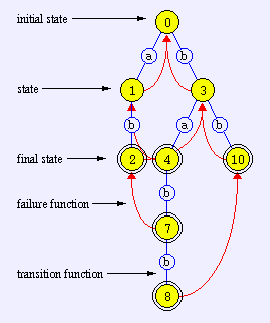
\includegraphics[width=8cm]{informatika/algoritmy_a_ds/obrazky/ahocorasick-automatron.png}\end{center}

Zložitosť vyhľadávania je lineárna vzhľadom k dĺžke textu a počtu nájdených \uv{slov} (pozn.: ten môže byť až kvadradický - slovník a, aa, aaa, aaaa; reťazec aaaa). Trie štruktúru je možné vyrobiť raz a potom používať počas vyhľadávania - uchovávame si najdlší match a používame suffix odkazy (aby sme udržali linearitu výpočtu).

Výstavba stromu se provede prostým zařazováním slov do trie-stromu podle prefixů. Na této struktuře je potom možné v lineárním čase (vzhledem k počtu znaků hledaných slov) předpočítat hodnoty failure funkce: automat vždy pustíme na sufix aktuálně zkoušeného slova, bez prvního znaku. Díky tomu, že průběžně ukládáme hodnoty nalezených slov, pro každé písmeno provede max. 2 kroky (postup vpřed a uložení hodnoty, kam bych spadnul).


\subsubsection*{Knuth-Morris-Pratt}

Obdoba Aho-Corasick, ale hľadá len jedno slovo. Samozrejme nie je potrebná dopredná funkcia (vždy iba nasledujúci znak), používa sa \uv{partial match} tabuľka (failure funkcia).

\begin{verbatim}
algorithm kmp_search:
    input:
        S (the text to be searched)
        W (the word sought)

    m = 0 (the beginning of the current match in S)
    i = 0 (the position of the current character in W)
    an array of integers, T (the table, computed elsewhere)

    while m + i is less than the length of S, do:
        if W[i] = S[m + i],
            i = i + 1
            if i equals the length of W,
                return m
        otherwise,
            m = m + i - T[i],
            if i is greater than 0,
                i = T[i]

    (if we reach here, we have searched all of S unsuccessfully)
    return the length of S
\end{verbatim}

Zložitosť algoritmu je je $O(k)$ (k je dĺžka S) - cyklus je vykonaný najviac $2k$ krát.

Algoritmus na výrobu tabuľky:
\begin{verbatim}
algorithm kmp_table:
    input:
        W (the word to be analyzed)
        T (the table to be filled)

    i = 2 (the current position we are computing in T)
    j = 0 (the zero-based index in W of the next
           character of the current candidate substring)

    (the first few values are fixed but different
          from what the algorithm might suggest)
    let T[0] = -1
    T[1] = 0

    while i is less than the length of W, do:
        (first case: the substring continues)
        if W[i - 1] = W[j],
            T[i] = j + 1
            i = i + 1
            j = j + 1

        (second case: it doesn't, but we can fall back)
        otherwise, if j > 0,
            j = T[j]

        (third case: we have run out of candidates. Note j = 0)
        otherwise,
            T[i] = 0
            i = i + 1
\end{verbatim}


Zložitosť tohoto algoritmu je $O(n)$ (n je dĺžka W) - cyklus skončí najviac po $2n$ iteráciách.
